%Every piece of package I've acumulated over the last years
%%%%%%%%%%%%%%%%%%%%%%%%%%%%%%%%%%%%%%%%%%%%%%%%%%%%%%%%%%%%%%%%%%%%%%%%%%%%%%%%%%%%%%%%%%%%%%
\documentclass[a4paper,12pt]{article}
\usepackage[utf8]{inputenc}
\usepackage{imakeidx}
\usepackage{graphicx}
\usepackage{float}
\usepackage{amsmath}
\usepackage[backend=bibtex,style=verbose]{biblatex}
\bibliography{bibliography}
\usepackage{csquotes}
\usepackage{tcolorbox}
\usepackage{multirow}
\usepackage{caption}
\usepackage{afterpage}
\usepackage[margin=1in]{geometry}
\usepackage[english,spanish]{babel}
\usepackage{tikz}
\usepackage{mwe}
\usepackage{circuitikz}
\usepackage{subcaption}
%%%%%%%%%%%%%%%%%%%%%%%%%%%%%%%%%%%%%%%%%%%%%%%%%%%%%%%%%%%%%%%%%%%%%%%%%%%%%%%%%%%%%%%%%%%%%%
\begin{document}
\title{Evaluación Continua de Mecánica II\\ Temas 2-3}
\author{Gabriel D'Andrade Furlanetto}
\maketitle 

\section{Péndulo de Foucault}

\subsection*{a) Escribe la segunda ley de Newton para el grave y demuestra que la tensión $\boldsymbol{T}$ se puede aproximar como $T \approx m\boldsymbol{g}_{ef}$, donde $\boldsymbol{g}_{ef}$ es la gravedad efectiva.}

\begin{figure}[H]
  \centering
  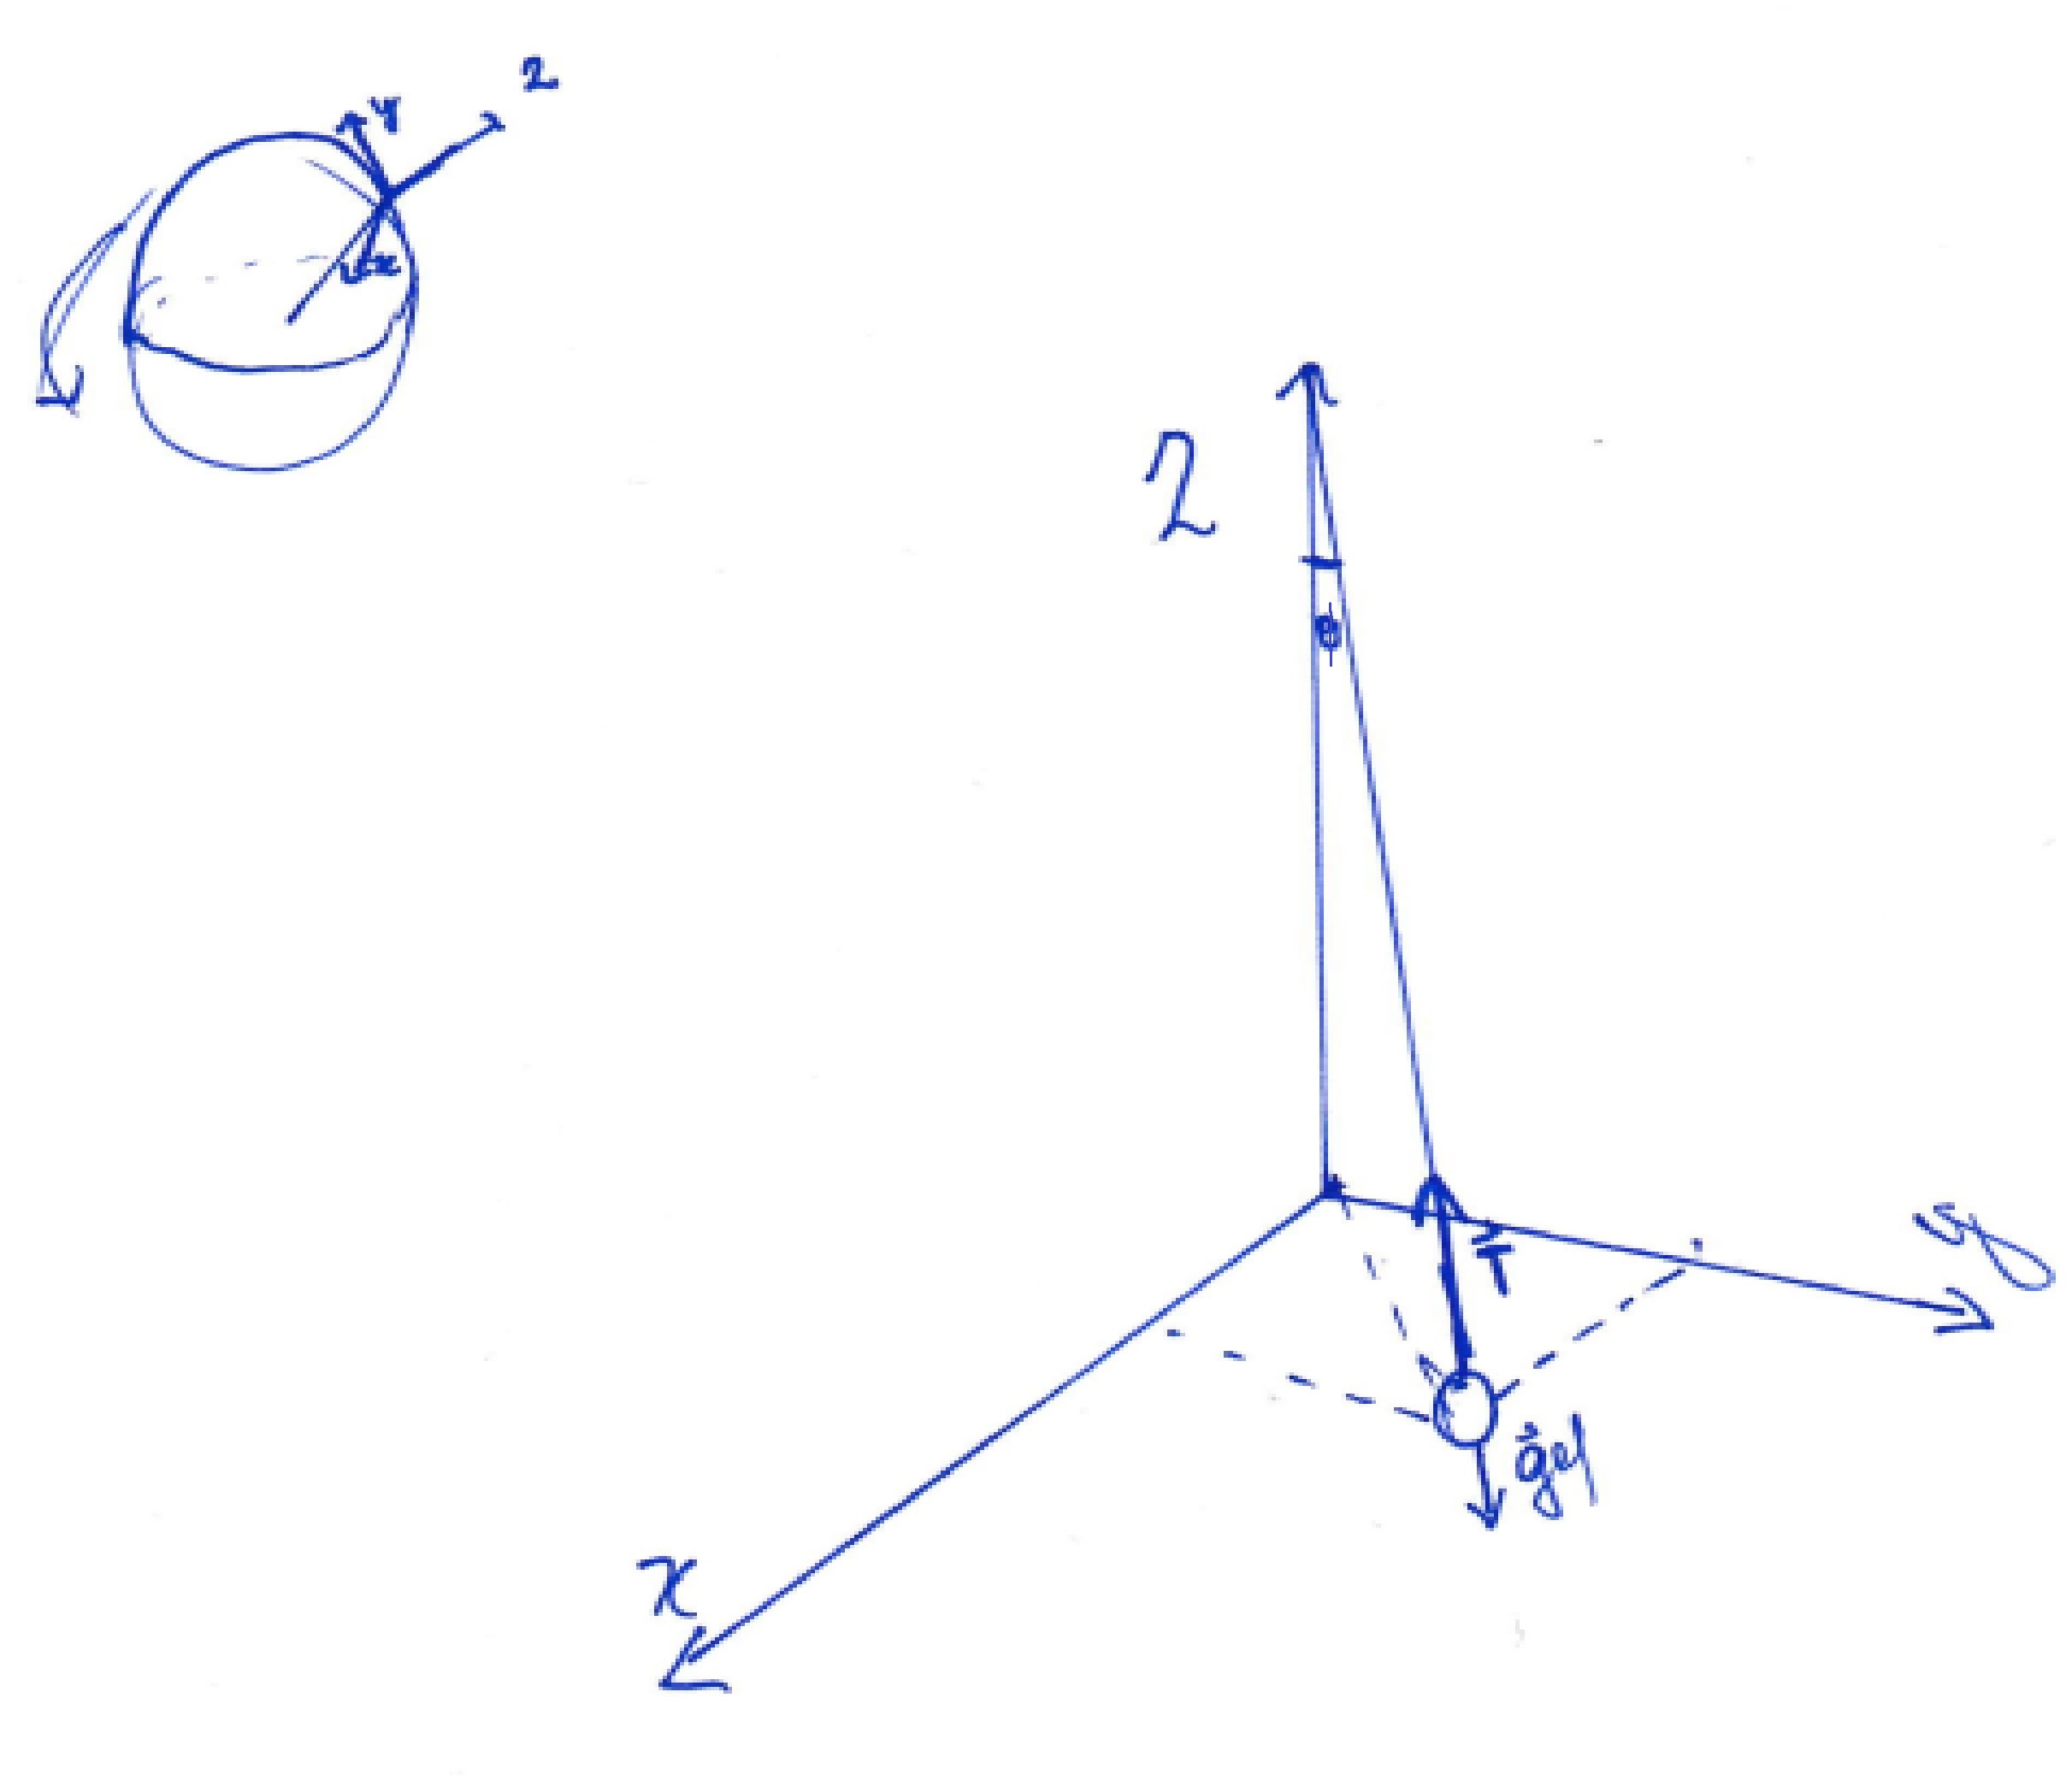
\includegraphics[width=0.5\textwidth]{foucault.jpg}
  \caption{Representación del problema}
  \label{fucas}
\end{figure}


Como estamos en el sistema de la Tierra, sabemos que podemos escribir la segunda Ley de Newton para este sistema como:

\begin{equation}
  m\ddot{\boldsymbol{r}} = \boldsymbol{F}_{ap} + \boldsymbol{F}_{cf} + \boldsymbol{F}_{cor}
\end{equation}

Para nuestro problema en particular, la fuerza aplicada será, por un lado, la tensión y, por otro, la gravedad. De esta manera, tendremos que:

\begin{equation}
  m \ddot{\boldsymbol{r}} = \boldsymbol{T} + m\boldsymbol{g} + m(\boldsymbol{\omega} \times \boldsymbol{r}) + 2m (\dot{\boldsymbol{r}} \times \boldsymbol{\omega})
\end{equation}

Esta ecuación se puede simplificar bastante si consideramos que el término centrífugo se puede combinar al gravitatorio y, al final, tendremos un término de la gravedad efectiva\footnote{Tomaremos esto simplemente como un hecho conocido, pero cualquier libro texto estándar de mecánica lo tiene tratado explícitamente.}:

\begin{equation}
  \label{initialus1}
  m \ddot{\boldsymbol{r}} = \boldsymbol{T} + m\boldsymbol{g}_ef + 2m (\dot{\boldsymbol{r}} \times \boldsymbol{\omega})
\end{equation}

Para proseguir en la resolución, tendremos que mirar el problema en concreto. Primeramente, podemos escribir que, en el eje $z$, la segunda ley de Newton tendrá forma aproximadamente\footnote{Aquí estamos aproximando la fuerza de Coriolis no tiene efecto en el eje $z$ y que partícula aproximadamente no se mueve   } 

$$T_{z} - mg_{ef} \approx 0$$

Por la figura \ref{fucas}, sabemos por trigonometría básica que $T_{z} = T \cos{\phi}$. Como estamos en el régimen de oscilaciones pequeñas en $\phi$, sabemos que:

\begin{equation}
  T_{z} \approx T
\end{equation}

Si juntamos las dos condiciones, tendremos que:

\begin{equation}
  T \approx m g_ef 
\end{equation}

Como queríamos demostrar.

\subsection*{b) Escriba las ecuaciones de movimiento del plano horizontal en forma matricial}

Como asumimos en nuestra aproximación que no había movimiento vertical, nos resta analizar el movimiento horizontal. Inicialmente, escribimos en coordenadas el término de Coriolis. Como $\dot{\boldsymbol{r}} = (\dot{x},\dot{y},\dot{z})$ y $\boldsymbol{\omega} = (0,\omega \sin\theta, \omega \cos\theta)$:

$$\boldsymbol{F}_{cor} = 2m (\dot{\boldsymbol{r}} \times \boldsymbol{\omega}) = 2 m (\dot{y}\omega \cos\theta-\dot{z} \sin\theta, -\dot{x}\omega \cos\theta, \dot{x} \omega \sin\theta )$$

Como ya lo decimos, vamos a ignorar el término vertical en este problema, entonces tomaremos el término de Coriolis como $\boldsymbol{F}_{cor}= 2 m (\dot{y}\omega \cos\theta, -\dot{x}\omega \cos\theta )$. Por la ecuación \eqref{initialus1}, si determinamos las tensiones determinaremos las ecuaciones de movimiento. Eso se puede hacer de manera casi trivial con un poco de trigonometría, de la que concluiremos que $\frac{T_x}{T} = -\frac{x}{\ell} $ y $\frac{T_y}{T} = -\frac{y}{\ell}$\footnote{El signo negativo es una sutileza que se puede fácilmente olvidar, pero viene del hecho de que la tensión estará siempre opuesta al movimiento. Si no lo fuera, la solución explotaría y eso claramente no es una solución física para un péndulo.}. De eso, concluimos que:
$$T_x = -\frac{mgx}{\ell} $$
$$T_y = -\frac{mgy}{\ell} $$

De manera que podemos escribir las ecuaciones de movimiento:
\begin{equation}
  \begin{aligned}
    \ddot{x} = -\frac{g x}{\ell} + 2\dot{y}\omega \cos\theta
    \ddot{y} = -\frac{g y}{\ell} - 2\dot{x}\omega \cos\theta
  \end{aligned}
\end{equation}

Que podemos escribir vectorialmente como:

\begin{equation}
  \ddot{\boldsymbol{\chi}} +A\dot{\chi} + B \boldsymbol{\chi} = 0
\end{equation}

Donde:
\begin{equation}
  \boldsymbol{\chi} = \begin{pmatrix} x \\ y\end{pmatrix} \qquad 
  A = 2\omega \cos\theta \begin{pmatrix} 0 & -1 \\ 1 & 0\end{pmatrix} \qquad
  B = \frac{g}{\ell} \begin{pmatrix} 1 & 0 \\ 0 & 1\end{pmatrix}
\end{equation}

Que era lo que queríamos encontrar.

\subsection*{c) Integre las ecuaciones de movimiento de manera exacta y demuestra que la órbita del grave es una elipse que precesa con velocidad angular $\omega \cos\theta$.}

Para integrar nuestra ecuación, utilizaremos la técnica que vimos en clases de introducir una variable compleja\footnote{Más que una coincidencia feliz, es casi siempre ideal introducir números complejos para tratar de rotaciones en $\mathbb{R}^{2}$, que es exactamente la esencia de nuestro problema, por el isomorfismo entre $SO(2)$ y $U(1)$.} , $z = x + i y $. Si sumamos la primera fila por $i$ veces la segunda. Lo hacemos explícitamente:

$$\ddot{x} + i\ddot{y} + 2\omega \cos\theta(\dot{y} -i \dot{x}) + \frac{g}{\ell} (x + i y) =\frac{d^2}{dt^2} \left(x + i y\right) + 2\omega \cos\theta\frac{d}{dt}-i (iy + x) + \frac{g}{\ell} (x + i y) = 0 $$

$$\ddot{z} - 2i\omega\cos\theta \dot{z} + \frac{g}{\ell} z = 0$$


\section{Cono con Canica}


\end{document}

